% Created 2015-11-29 Sun 21:51
\documentclass[11pt]{article}
\usepackage[utf8]{inputenc}
\usepackage[T1]{fontenc}
\usepackage{fixltx2e}
\usepackage{graphicx}
\usepackage{longtable}
\usepackage{float}
\usepackage{wrapfig}
\usepackage{rotating}
\usepackage[normalem]{ulem}
\usepackage{amsmath}
\usepackage{textcomp}
\usepackage{marvosym}
\usepackage{wasysym}
\usepackage{amssymb}
\usepackage{hyperref}
\usepackage{xcolor}
\usepackage{titling}
\setlength{\parindent}{0em}
\setlength{\droptitle}{-40pt}
\setlength{\parskip}{1em}
\posttitle{\par\end{center}}
%\posttitle{\par\end{center}\vskip -3em}

\usepackage[margin=1in,footskip=0.25in]{geometry}
\setcounter{secnumdepth}{2}
\title{CS 444: Artificial Intelligence \\ Section 1 \\ James Madison University \\ Spring 2021 (3 credits)}
 \hypersetup{
  colorlinks=true, linkcolor=blue,
  linkbordercolor=red,  pdfborderstyle={/S/U/W 1}
}

\date{\vspace{-5ex}}

\begin{document}

\maketitle

\section{Basic Course Information}
                                        
\subsection{Course Description and Goals}
What is intelligence?  Is it possible for a computer to possess intelligence or be intelligence?  How do we measure this quality about a non-human, or
inanimate object? \\

In this class, we will explore methods to solve problems that seemingly require intelligence, focusing on problems where the best known algorithms
we have to ``solve" the problem are intractable.  We will then proceed to develop knowledge bases, that is, sets of facts that, allow for computations
to infer new facts from existing ones.  Finally, we will focus on utilizing a probabilistic representation of the world, so that we can develop
more advanced intelligent ``agents".
 
\subsection{Meeting Times and Locations}
\begin{center}
\begin{tabular}{cccc}
Section & Days & Time &  Location\\
\hline
01 & T/R & 11:20-12:35  & Zoom \\
\end{tabular}
\end{center}

\subsection{Instructor}
\label{instructor}
\begin{center}
\begin{tabular}{rl}
\emph{Name} & Dr. Kevin Molloy\\
\emph{Office} & ISAT/CS  216\\
\emph{Email} & molloykp@jmu.edu\\
\emph{Office Hours} & T 16:30 - 18:30 \\
                                 & W  14:00 - 16:00 \\
                                 & R 13:00 - 14:00 \\
\end{tabular}
\end{center}

\subsection{Website: \href{https://w3.cs.jmu.edu/molloykp/teaching/cs444/cs444\_2021Spring}
                                          {https://w3.cs.jmu.edu/molloykp/teaching/cs444/cs444\_2021Spring}}
Much of the information for this course will be disseminated via this website.  You should
check this website often (at least once a week) for announcements and updates.
                           
\subsection{Prerequisites}
A grade of ``C-'' or better in {\bf CS 327 (discrete structure II)}. 




\subsection{Required Texts}
\begin{minipage}{0.3\textwidth}
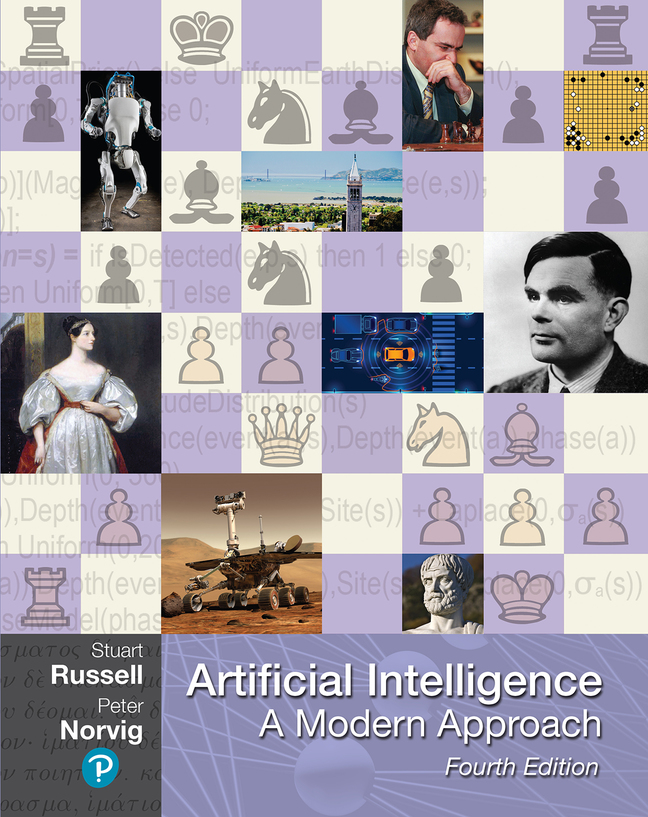
\includegraphics[width=\linewidth]{RusselNorvigTextbookImage4thED.jpg}
\end{minipage}
\begin{minipage}{0.6\textwidth}
\emph{{\bf Artificial Intelligence: A Modern Approach, Forth Edition}} \\by  Stuart Russell and Peter Norvig.
\end{minipage}


\subsection{Computing Resources}
You will require access to a computer for this class.  A machine running Windows, Mac OS, or 
Ubuntu/Linux will work fine.  My opinion is that Mac OS and Ubuntu/Linux machines are easier
to use. Information is available on the website on how to utilize a virtual machine that will
supply all the software you will need for this class (and provide a common 
environment to what you will experience in the labs). 

\newpage 

\subsection{Expectations/Keys to Success}
\subsubsection{Homework}
 In a three-hour course, you should expect \textbf{six hours} of homework per week.
 How you manage your schedule is up to you, but do spend some time each day on this course. 

\subsubsection{Preparing for Class}
Material will be introduced in class and 
then reinforced with reading and/or assigned videos.  
You will have a take home \textbf{quiz} almost every week (12 of them).

\subsubsection{Programming Assignments} 
Programming assignments (PA) will utilize the python programming language.  
Each assignment can take about between 4 and 8 hours to complete.
Don't wait until the week before the assignment is due to get started. 

\subsubsection{Seeking Help}
Piazza is a great platform to see help in this class.  However, I generally
 do {\bf not} answer Piazza questions over the weekend.
If  you  choose  to  complete  assignments  at  the  last  minute  or  after  the deadline, 
please keep this in mind.  I will make sure
any questions posted over the weekend are answered on Monday.  
Please ask questions using Piazza first if at all possible. I have it set up so that I get an email 
when a question is posted to Piazza, 
so emailing me is not quicker and by posting to Piazza you will have a chance of being answered by a classmate, 
TA, or another faculty member.  Email should be reserved for questions whose answers
would only benefit you personally or only I would know the answer to.


\subsection{Communication}
We will use a number of different tools for communication in this course.  
These include:
\begin{itemize}
\item \href{https://w3.cs.jmu.edu/molloykp/teaching/cs444/cs444\_2021Spring/}{https://w3.cs.jmu.edu/molloykp/teaching/cs444/cs444\_2021Spring/} is our central course web site. The announcements, discussion
board, videos, and documents posted there are part of the required reading
for the course.
\begin{itemize}
\item Use public posts on Piazza to discuss the material related to this course.
\item \textbf{Canvas} will be used to submit assignments and disseminate grades
\item \textbf{Mail the professor} if you have logistic or
personal issues to discuss such as setting up an appointment
outside of office hours, if a health problem arises, or if you
have a personal emergency.
\end{itemize}
\item \textbf{Office Hours}  No appointments are required to attend office
hours or you can make an appointment with me.
\end{itemize}

\subsection{Attendance and Participation}
Regular attendance and fully engaged participation is expected.  Your grade will be partially 
based on in-class activities, so, attendance will affect your grade.

\emph {Please silence your cell phone while class is in session and mute your Zoom session 
while not asking questions/interacting with others.}. 

I strongly encourage you to check the main website and the Piazza web forum regularly for important
announcements (usually regarding programming projects). You may also use the Piazza forum to ask 
general questions of interest to the class as a whole (e.g., administrative issues or project clarification questions) as 
well as to offer each other general advice on class assignments. However, do not post any information that would 
violate the university academic integrity policy. If you are unsure about this, please email me for approval before you post. 


\section{Methods of Evaluation and Grading Policies}

You are responsible for all material discussed in lecture and discussion section and posted on the 
class web page, including announcements, deadlines, policies, etc. 

Your final course grade will be determined according to the following percentages: 
\begin{center}
\begin{tabular}{l|r|r}
\hline \hline
Component  &  Count & Weight\\
\hline
Weekly Mastery Quizzes             &  12                                    & 50\% \\ \hline
Homework/Labs, Participation     &  6 to 8                              & 15\% \\ \hline
Programming Assignments          &  6 to 8                             & 35\%\\ \hline
\hline
\end{tabular}
\end{center}

Letter grades will be assigned on the scale A=90-100, B=80-89, C=70-79, D=60-69, F=0-59, 
with potential minor adjustments after considering the overall performance of the class and 
actual distribution of numeric scores. I will use {\bf +} and {\bf- } grades at my discretion.  

\subsection{Mastery Quizzes instead of Exams}
There will {\bf}not be a midterm and final exam in this class.  Instead, 50\% of your
grade will be comprised of mastery quizzes.
Almost each week, you will be quizzed on the material from the past 2 sessions of class.
If you have mastered the material and are happy with your grade, you are done.
If you want another chance, a second quiz (on the same material) will be given the following week.
Thus, if you are retaking the quiz, you would have 2 quizzes that week.  
Quizzes will be timed to 25 minutes each and sized appropriately.

Halfway though the semester, the quizzes will begin to have 1 or 2 questions
from prior sections as well.  These quiz that address prior topics will be announced at least 1 week
before to allow for proper preparation.  

\subsection{Grading Disputes}
If you believe I have made an error while grading your work or calculating your final score, please 
bring it to my attention after class or during office hours. If I determine that there has been a simple mistake,
I will fix it immediately and no formal request is necessary. 

If you believe an exam question or assignment has been graded unfairly, you 
must submit a written formal request for a regrade via email.
Such requests 
must be submitted within one week of when the assignment in question is returned to you. 
\textcolor{red}{\emph Any coursework submitted for reconsideration may be regraded in its entirety, which could result 
in a lower score if warranted.}

\section{Course Policies}
Important announcements will be made in class and/or on the class website. Please make it a habit to check the web page and or your email daily during the week. 

Although every effort has been made to be complete and accurate, unforeseen circumstances arising during the semester could require the adjustment of any material given here. Consequently, given due notice to students, I reserve the right to change any information on this syllabus or in other course materials.

You are permitted to use course materials for your own personal use only. Course materials may not be distributed publicly or provided to others (excepting other students in the course), in any way or format unless explicitly allowed. 


\subsection{Programming Assignments(PA's)}
PA's must be submitted electronically following the instructions given in class and on the website.
Assignments may not be submitted by any 
other means (e.g., do not email your projects to me unless I request that). It is your responsibility to test your 
program and verify that it works properly before submitting it.

\subsection{Missed and Late Assignment Policy}
It will not be possible to receive credit for in-class work or mastery quizzes that are 
missed due to absence except in the case of
prearranged absences for sports, academic conferences, or other CS related activities.  Missing class
for these reasons requires coordination with me prior to missing class (no consideration will be given for
coordinating this after the missed class).

Programming assignments may be submitted up to 48 hours late for a 10\% penalty per 24-hour period. For example, a submission that would have
earned 90 points in an on-time submission will earn 90 x 0.90 = 81 points if submitted up to 24 hours late, or 90 x 0.80 = 72 points 
if submitted up to 48 hours late. If you make multiple submissions, I will typically grade the latest submission. If you wish me 
to grade a different submission, you must indicate this before the 48-hour late period is over. 

Regardless of the above policy, I reserve the right to refuse to grade any programs 
submitted after the beginning of the second class period following the project deadline, 
because I may discuss the solution in class. 

Project extensions will not necessarily be granted due to server congestion, system problems, network problems, 
power outages, etc., so do not wait to submit a program until the night it is due. 
No consideration in grading will be made for errors made in transferring files or submitting the wrong version of your project. 
Having a working, non-submitted version will not count; only submitted code will be be counted. 

You will be responsible for developing your own techniques for testing your projects before 
submitting it. I will grade your assignment based on test cases not provided to you in advance. 
Your code will be graded on a combination of correctness, completeness, documentation, and code style. 

I will be exploiting electronic methods to detect plagiarism
(this is an AI class, so, be aware that machine learning methods will be used).  
You should be able to explain your code to me.  
See Section \ref{sec-5-1} for more details.



\subsection{Adding and Dropping the Course}

Students are responsible for adding and dropping the course and verifying
these actions in \mbox{MyMadison}.   The last date to
drop this class with a "W" grade is March 19th.  
Please consult the appropriate 
\href{https://www.jmu.edu/registrar/students/print_dates.shtml}{registrar dates} for other deadlines as these dates
can change, especially with the current COVID-19 circumstances.
I will not give {\bf ``WP''}  or {\bf ``WF''} grades to students requesting a drop after the deadline except in extraordinary circumstances. 

\subsection{Disability Accommodations}
If you need an accommodation based on the impact of a disability, you must contact 
the \href{https://www.jmu.edu/ods}{Office of Disability Services} if you have not previously done so. 
Disability Services will provide you with an Access Plan letter that will verify your need for services and make recommendations 
for accommodations to be used in the classroom. Once you have shown me this letter, we will sit down and review the 
course requirements, your disability characteristics, and your requested accommodations to develop an individualized plan 
appropriate for this course. I will not make any accommodations without the appropriate documentation, as I am not 
qualified to diagnose disabilities. 

\subsection{Excused Absences}
All University's policies apply during the semester.  Some of these policies appear in the
Undergraduate Catalog.

Missing a mastery quiz for reasons such as illness, religious observance, participation in required university activities, or family or personal emergency (such as a serious automobile accident or the funeral of a close relative) all are circumstances that \textit{may} qualify as an excused absence.  
Where possible you should attempt by all means necessary to attend and take exams at their regularly scheduled class period.  

If you must be absent during an exam for a legitimate reason, you must contact me
 at least one week beforehand to make special
arrangements. Failure to make prior arrangements for a missed exam will result in a zero grade.
Excused absences will be granted at my discretion and only with appropriate documentation. 
Please contact me as soon as possible if you wish to request an excused absence.


Observance of religious events will be accommodated for students of any
faith.


\subsection{Classroom Behavior}
Students are expected to maintain a high level of civility for all
participants in and out of class meetings.  This includes respecting
the beliefs of participants of all genders, ethnicities, and social
backgrounds.  Harassment of any type will not be tolerated and failure
to behave in a respectful manner will result in referrals to
University Counseling or the Office of Student Judicial Affairs.  Any
instances of sexual harassment will be reported to the Office of Equal
Opportunity according the following policy:

\url{https://www.jmu.edu/JMUpolicy/policies/1340.shtml}


\subsection{Inclement Weather}
This class will operate in accord with JMU"s inclement weather policy
available at \\ 
 \href{http://www.jmu.edu/JMUpolicy/1309.shtml}{http://www.jmu.edu/JMUpolicy/1309.shtml}.  

\subsection{Religious Observation Accommodations}
I will give reasonable and appropriate accommodations to students requesting them on grounds of religious observation. 
If you require such accommodations you must notify me at least two weeks in advance.
 
.

\section{Academic Honesty and Collaboration}

\subsection{Academic Honesty}
You are expected to comply with the JMU Honor Code as stated in the Student Handbook and available from the 
\href{http://www.jmu.edu/honorcode}{Honor Council website} on all assignments, projects, and exams. 

Consulting with other students about problems and solutions is not necessarily a violation of the honor code, depending on the particular assignment. All final work turned in for an assignment must be your own unless it is a group project. In particular, you may not share source or binary code on programming assignments unless the project specification explicitly allows it. If you are in doubt about whether something is an honor code violation, please contact me immediately. 

If I find evidence of a violation of the honor code, I will bring the matter to the attention of the involved individuals via email and request a face-to-face meeting. As per section IV of the honor code, first time student offenders may agree that a violation has occurred and accept an appropriate penalty by submitting an "Informal Resolution Agreement Form" to the honor council. If the student is not a first-time offender or if there is disagreement about the violation or penalty, the matter will be referred to the honor council 
under section V of the honor code. 


\subsection{PRIME DIRECTIVE}
\label{sec-5-1}
\textbf{\label{PRIME-DIRECTIVE}PRIME DIRECTIVE: Be able to explain your own work including homework code and exam solutions.}

Nearly all cheating in programming can be averted by adhering to the
PRIME-DIRECTIVE. Students may be asked at any time to explain code
or exam solutions they submit.  Inability to do so will be construed
as evidence of misconduct.  More specific guidelines are given below.

\subsubsection{Thou Shalt Not}
\label{sec-5-2}
For the purposes of this course, the following actions constitute
scholastic misconduct (cheating):
\begin{itemize}
\item Directly copying someone else's solution to a homework problem,
including student solutions from a previous semester
\item Directly copying an answer from some outside source such as the
Internet or friend for a homework problem
\item Making use of an Instructor Solution manual to complete homework
problems
\item Paying someone for a homework solution or submitting someone else's
work as your own
\item Posting solutions to any web site including our course web site
\item Collaborating or copying someone else's answer during an exam
\item Aiding or abetting any of the above
\item Witnessing any of the above and failing to report it the instructor
immediately
\end{itemize}

\subsubsection{Fair Collaboration}
The purpose of this course is to learn about programming and learning
from one another is a great help.  To that end, the following actions
\textbf{will NOT be considered cheating in this course.}
\begin{itemize}
\item Talking to other students in the course about HW problems and
informally describing how a problem may be solved.
\item Getting or giving help fixing a bug or two: a second set
of eyes is a great boon to finding that misplaced semicolon that is
preventing your code from compiling.
\item Searching the Internet for alternative presentations of a
programming concept.
\item When unsure whether collaboration is fair or not, stop the activity
until it can be cleared with instructor.
\end{itemize}


\subsection{Penalties}
\label{sec-5-3}
Any instance of misconduct will be referred to the
honor board.

\section*{Acknowledgments}
Many of the course materials we will be using this semester, including portions of this syllabus, were developed by other 
faculty members in the JMU Computer Science department and from the book's authors.
Contributors include: Nathan Sprague, Zoran Duric, and Amarda Shehu.
%
%
\end{document}